% Chapter Template

\chapter{Ensayos y resultados} % Main chapter title
En este capítulo se presentan las pruebas realizadas sobre el prototipo de pruebas del sistema. Se detallan los procedimientos para probar los modelos para detección facial, el sensor de movimiento, el consumo energético del sistema y los servicios en la nube empleados.

\label{Chapter4} % Change X to a consecutive number; for referencing this chapter elsewhere, use \ref{ChapterX}

%----------------------------------------------------------------------------------------
% SECTION 1
%----------------------------------------------------------------------------------------
\section{Banco de pruebas}
Para llevar a cabo pruebas y mediciones precisas sobre el sistema, fue necesario montar un conjunto de herramientas e instrumentos para evaluar su funcionamiento. El banco de pruebas utilizado para este trabajo es el que se muestra en la figura \ref{fig:test_bench}.

\begin{figure}[h]
	\centering
	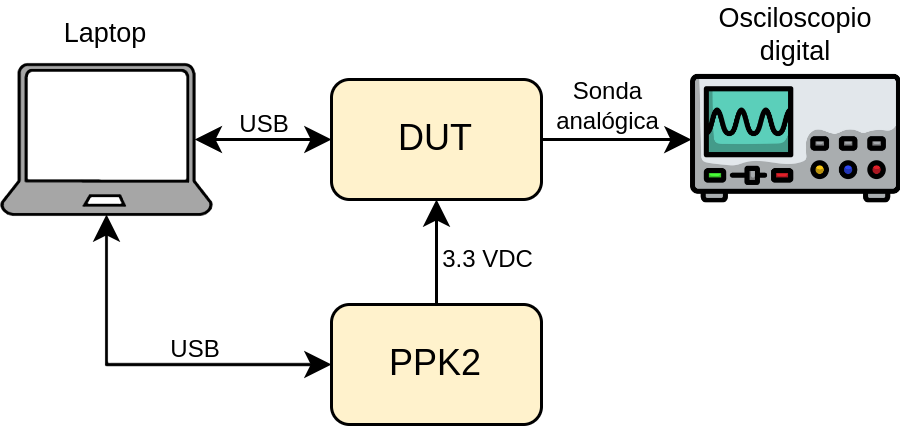
\includegraphics[scale=0.3]{./Figures/test_bench.png}
	\caption{Banco de pruebas.}
	\label{fig:test_bench}
\end{figure}

Los componentes que conforman el banco de pruebas según la figura \ref{fig:test_bench} son:
\begin{itemize}
	\item Laptop: cumple la función de ejecutar el software necesario para ejecutar las pruebas, monitorear y controlar todos los periféricos conectados mediante USB.
	\item Osciloscopio digital: TDS200C de Tektronix, es el instrumento utilizado para visualizar y medir las señales eléctricas generadas por el sistema. Su función principal para este trabajo fue evaluar las señales generadas por el sensor de movimiento.
	\item PPK2: Power Profiler Kit 2 de Texas Instruments, es un \textit{datalogger} enfocado en la medición de corrientes muy pequeñas y sirivió para evaluar el consumo de corriente cosumido por el dispositivo.
	\item DUT: es el prototipo de pruebas en sí, sobre este se realizan todas las pruebas y mediciones con todos las herramientas del banco de pruebas.
\end{itemize}

%----------------------------------------------------------------------------------------
% SECTION 2
%----------------------------------------------------------------------------------------
\section{Pruebas sobre los modelos}
Estas pruebas tuvieron el objetivo de ensayar el \textit{pipeline} donde se encuentran los modelos de MTCNN para detección facial obtenidos para TensorFlow, TensorFlow Lite sin cuantización y TensorFlow Lite con cuantización a 8 bits y TensorFlow Lite Micro con cuantización a 8 bits. La figura \ref{fig:test_image} presenta una imagen que contiene 3 rostros de formato RGB888 y dimensiones 96x96 píxeles, que fue utilizada como entrada para los \textit{pipelines} a probar.

\begin{figure}[h]
	\centering
	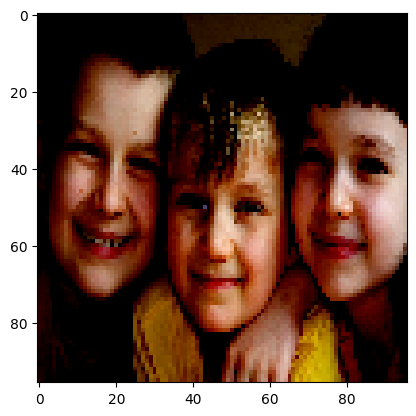
\includegraphics[scale=0.75]{./Figures/test_image.png}
	\caption{Imagen de prueba para los modelos.}
	\label{fig:test_image}
\end{figure}

Para probar los modelos para TensorFlow, TensorFlow Lite sin cuantización y TensorFlow Lite con cuantización a 8 bits, se utilizó Google Colab en conjunto con el \textit{framework} TensorFlow en lenguajes Python y varias bibliotecas para visualización de imágenes. En las figuras \ref{fig:test_tf_pnet}, \ref{fig:test_tf_rnet} y \ref{fig:test_tf_onet} se muestran los resultados obtenidos.

\begin{figure}[!htpb]
     \centering
     \begin{subfigure}[b]{0.28\textwidth}
         \centering
         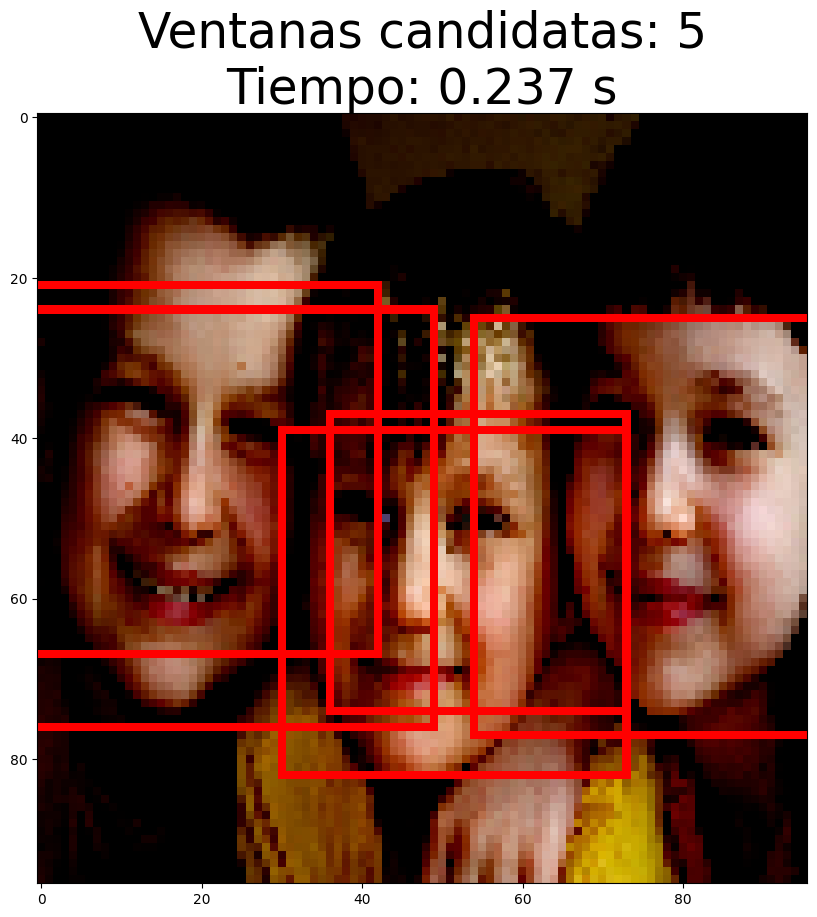
\includegraphics[width=\textwidth]{./Figures/test_tf_pnet_a.png}
         \caption{P-Net postprocesado.}
         \label{fig:1de3}
     \end{subfigure}
     \hfill
     \begin{subfigure}[b]{0.28\textwidth}
         \centering
         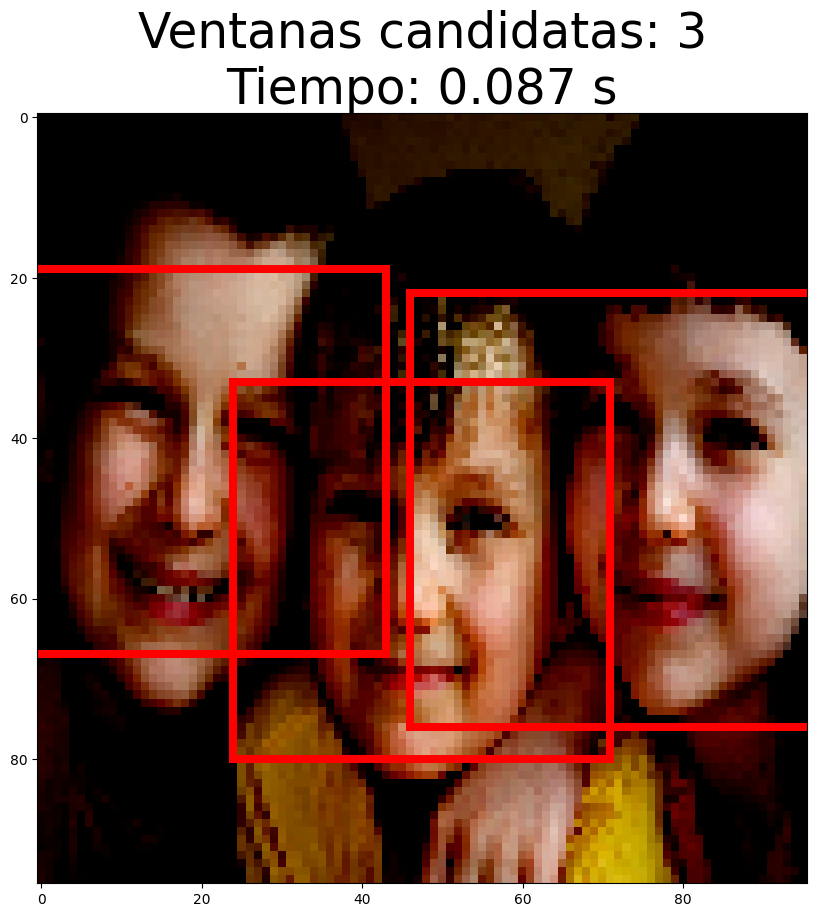
\includegraphics[width=\textwidth]{./Figures/test_tf_rnet_a.png}
         \caption{R-Net postprocesado.}
         \label{fig:2de3}
     \end{subfigure}
     \hfill
	 \begin{subfigure}[b]{0.28\textwidth}
         \centering
         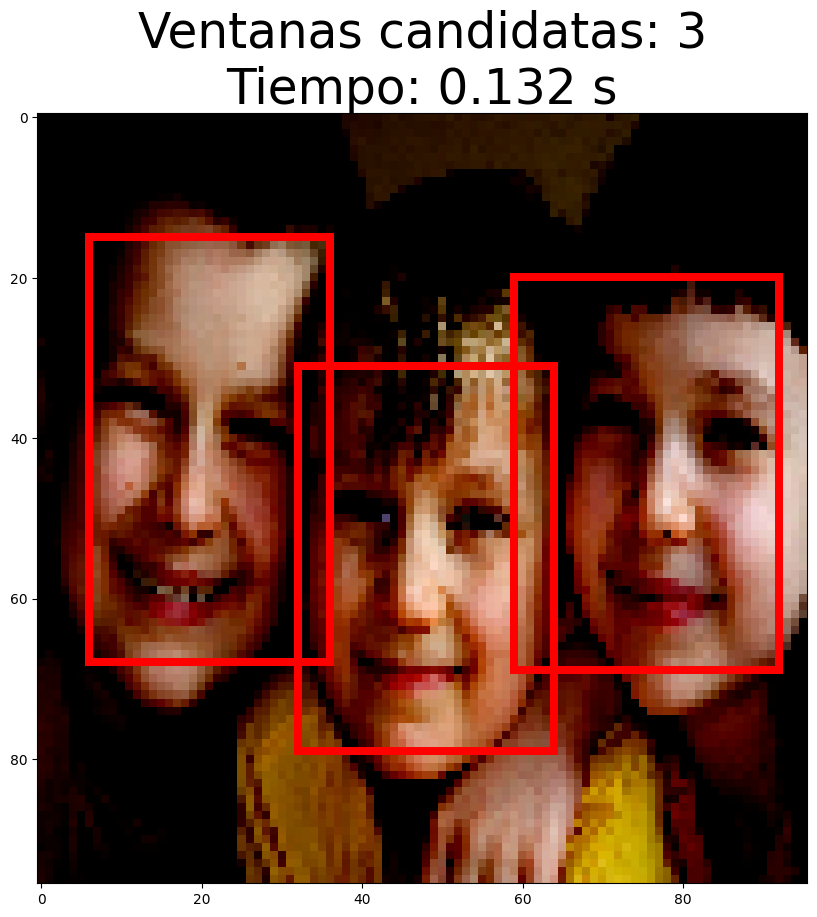
\includegraphics[width=\textwidth]{./Figures/test_tf_onet_a.png}
         \caption{O-Net postprocesado.}
         \label{fig:2de3}
     \end{subfigure}
     \hfill
        \caption{Resultados para TensorFlow.}
        \label{fig:test_tf_pnet}
\end{figure}

\clearpage


\begin{figure}[!htpb]
     \centering
     \begin{subfigure}[b]{0.28\textwidth}
         \centering
         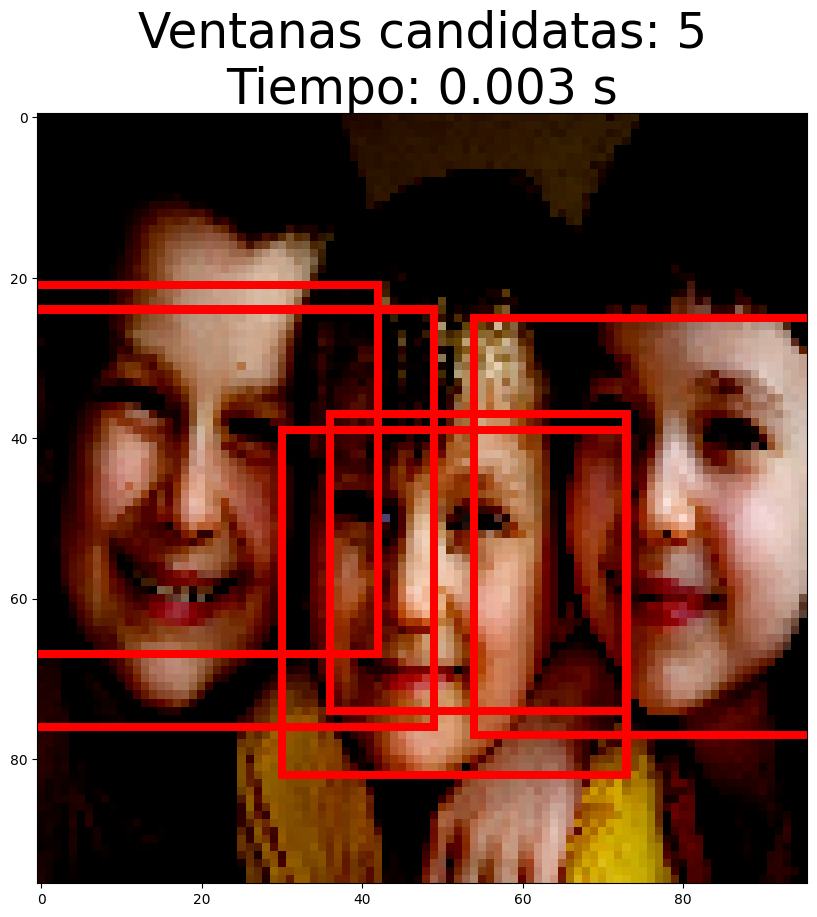
\includegraphics[width=\textwidth]{./Figures/test_tf_pnet_b.png}
         \caption{P-Net postprocesado.}
         \label{fig:1de3}
     \end{subfigure}
     \hfill
     \begin{subfigure}[b]{0.28\textwidth}
         \centering
         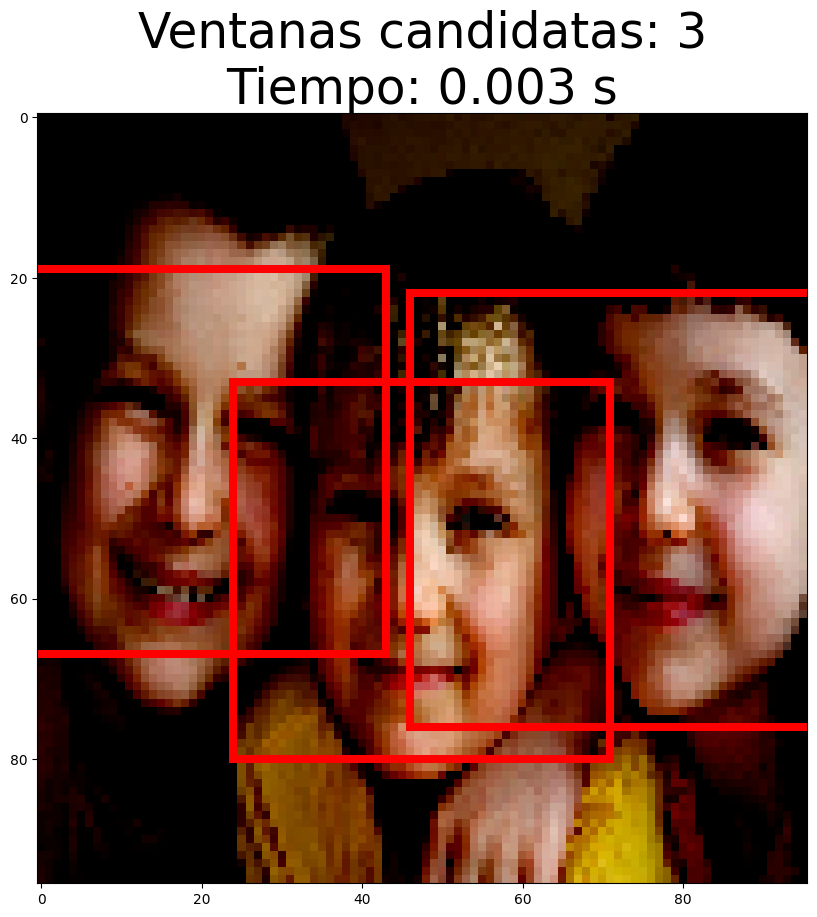
\includegraphics[width=\textwidth]{./Figures/test_tf_rnet_b.png}
         \caption{R-Net postprocesado.}
         \label{fig:2de3}
     \end{subfigure}
     \hfill
	 \begin{subfigure}[b]{0.28\textwidth}
         \centering
         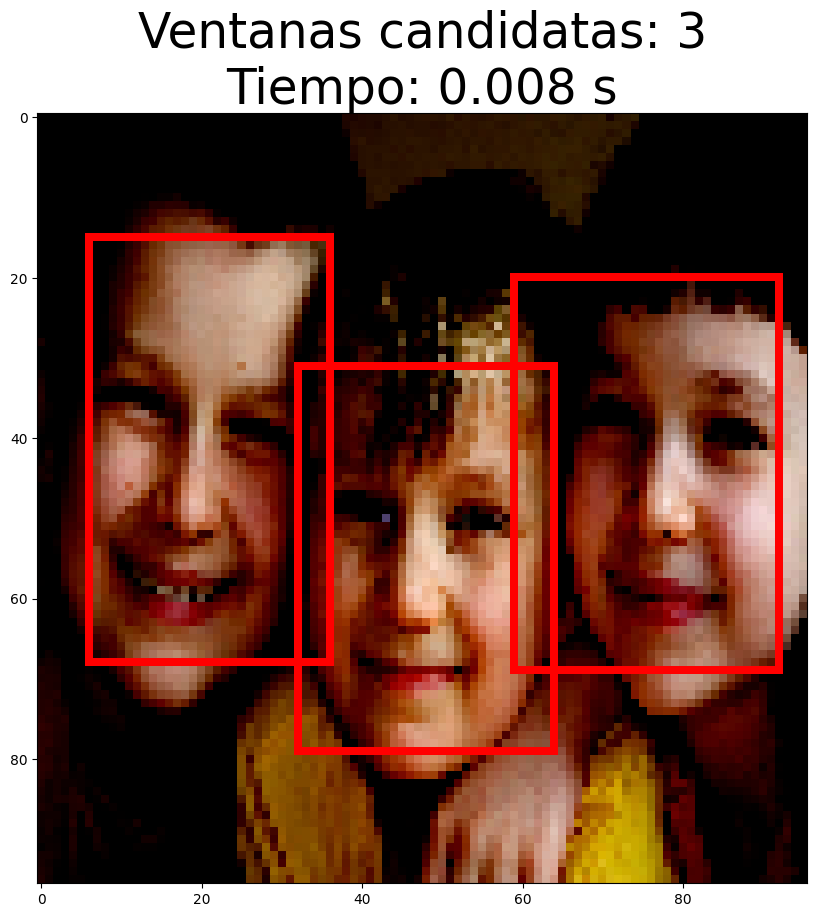
\includegraphics[width=\textwidth]{./Figures/test_tf_onet_b.png}
         \caption{O-Net postprocesado.}
         \label{fig:2de3}
     \end{subfigure}
     \hfill
        \caption{Resultados para TensorFlow Lite sin cuantización.}
        \label{fig:test_tf_rnet}
\end{figure}

\begin{figure}[!htpb]
     \centering
     \begin{subfigure}[b]{0.28\textwidth}
         \centering
         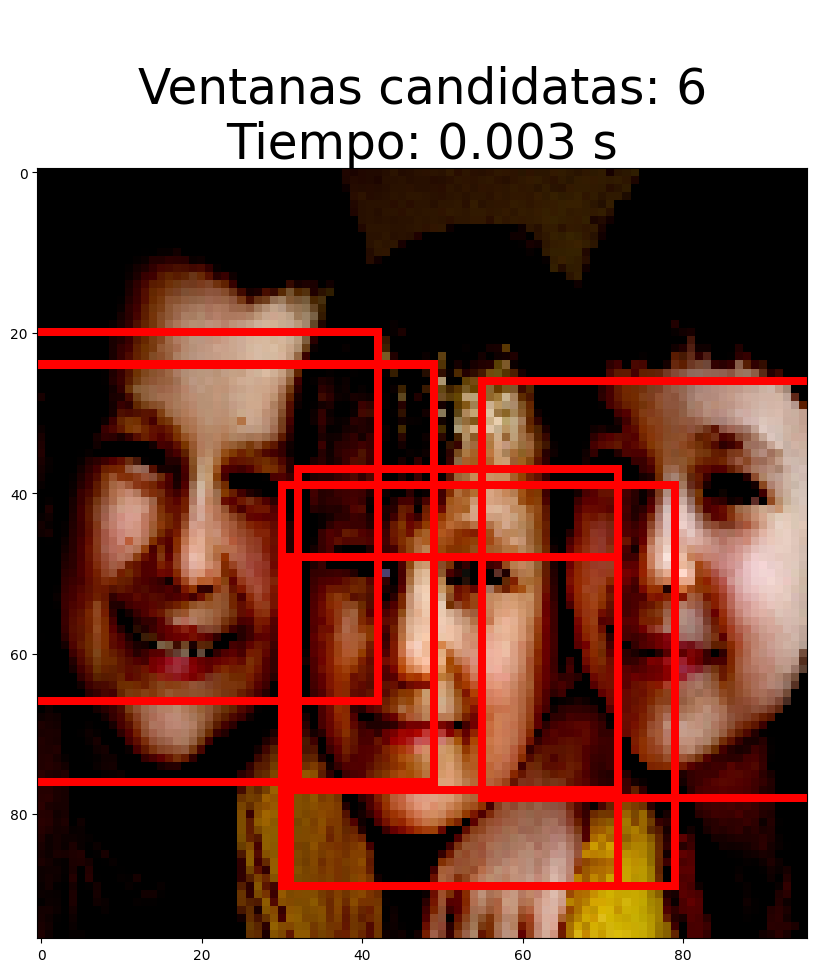
\includegraphics[width=\textwidth]{./Figures/test_tf_pnet_c.png}
         \caption{P-Net postprocesado.}
         \label{fig:1de3}
     \end{subfigure}
     \hfill
     \begin{subfigure}[b]{0.28\textwidth}
         \centering
         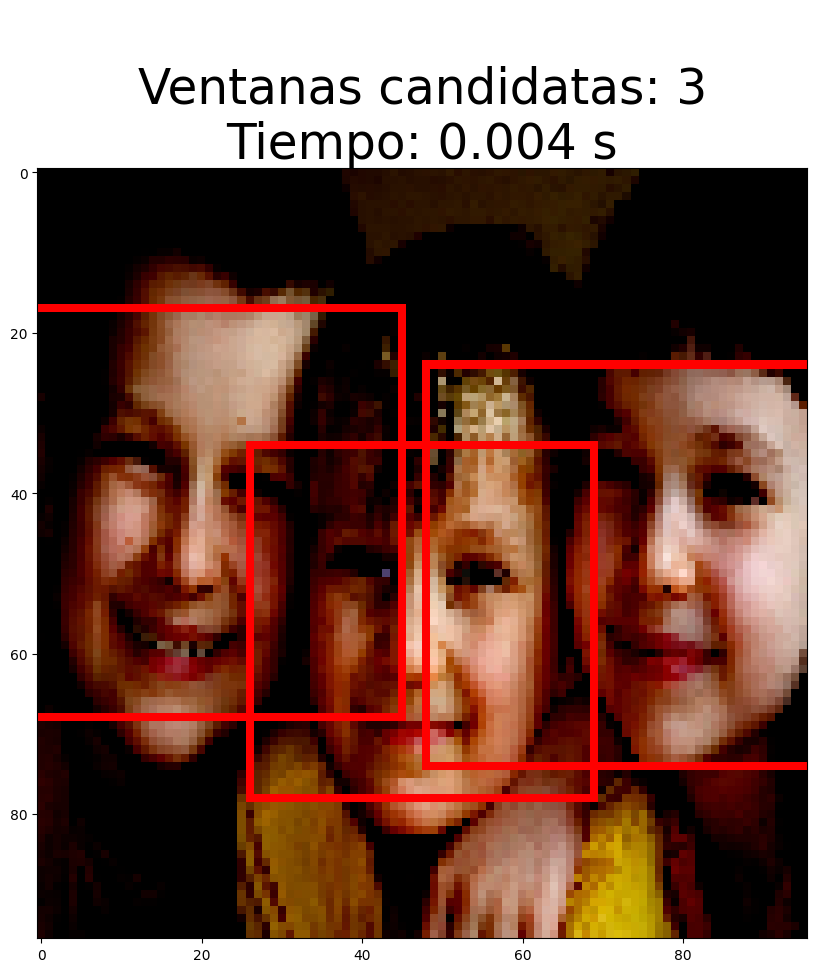
\includegraphics[width=\textwidth]{./Figures/test_tf_rnet_c.png}
         \caption{R-Net postprocesado.}
         \label{fig:2de3}
     \end{subfigure}
     \hfill
	 \begin{subfigure}[b]{0.28\textwidth}
         \centering
         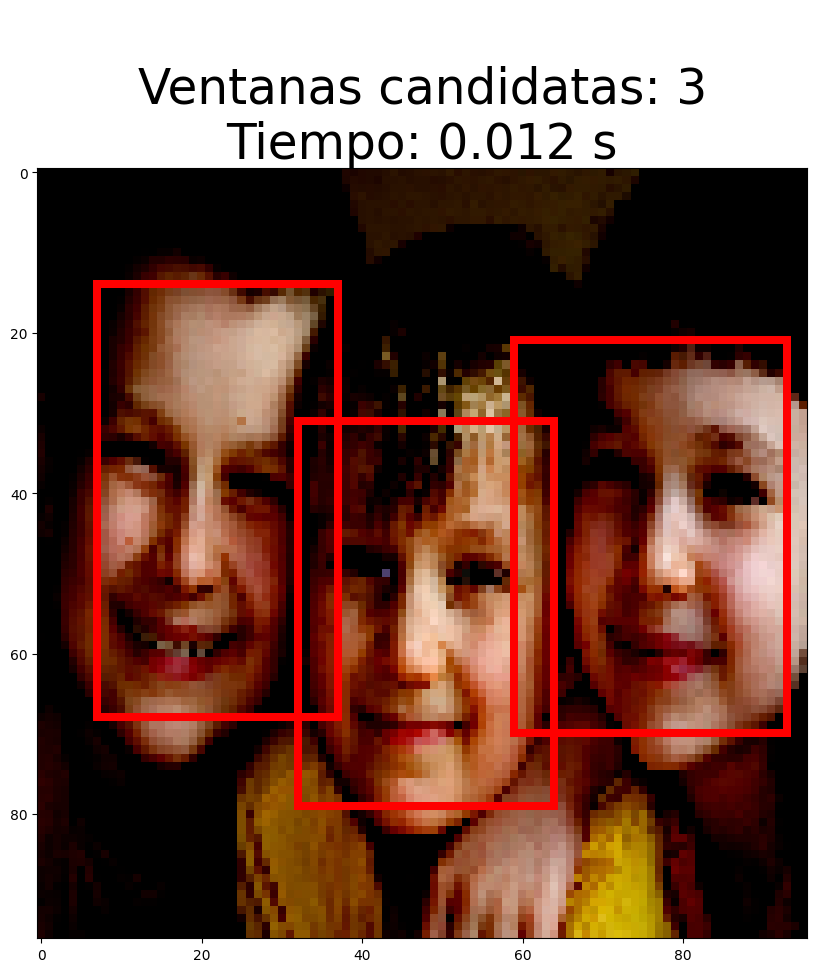
\includegraphics[width=\textwidth]{./Figures/test_tf_onet_c.png}
         \caption{O-Net postprocesado.}
         \label{fig:2de3}
     \end{subfigure}
     \hfill
        \caption{Resultados para TensorFlow Lite con cuantización a 8 bits.}
        \label{fig:test_tf_onet}
\end{figure}

Para probar el \textit{pipeline} y los modelos de MTCNN para TensorFlow Lite Micro con cuantización a 8 bits, se modificó el \textit{firmware} del prototipo de pruebas para que la imagen de prueba esté embebida en el binario de la aplicación y pueda ser leída dentro del programa. En la figura \ref{fig:test_tflm} se observan los resultados de esta prueba.

\begin{figure}[!htpb]
     \centering
     \begin{subfigure}[b]{0.28\textwidth}
         \centering
         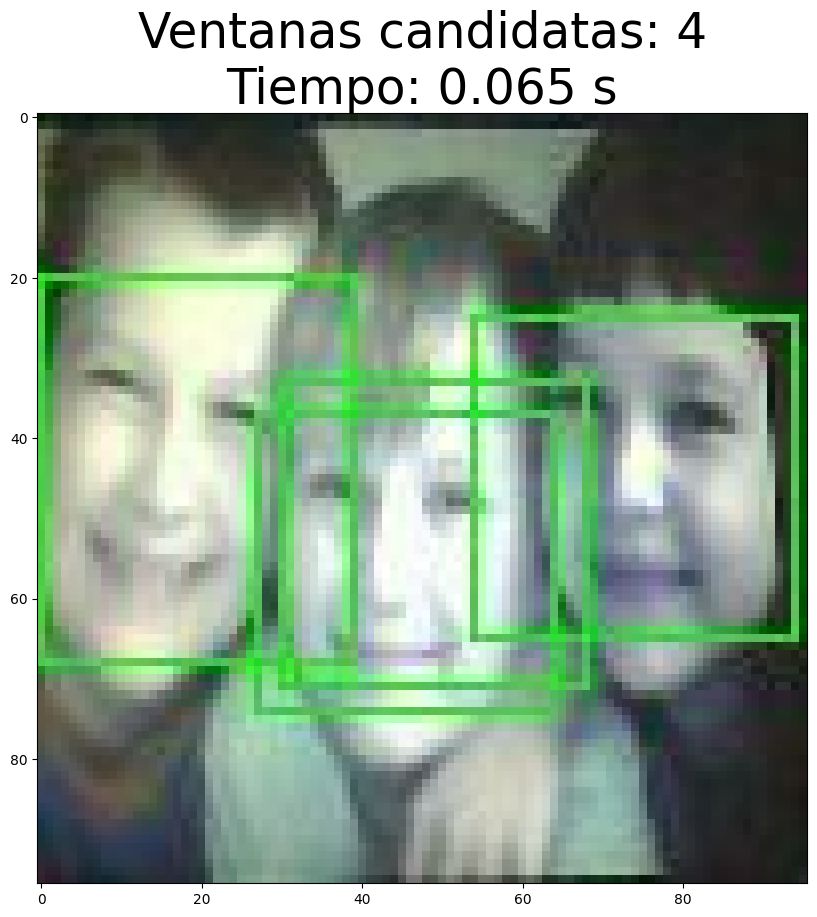
\includegraphics[width=\textwidth]{./Figures/pnet.png}
         \caption{P-Net postprocesado.}
         \label{fig:1de3}
     \end{subfigure}
     \hfill
     \begin{subfigure}[b]{0.28\textwidth}
         \centering
         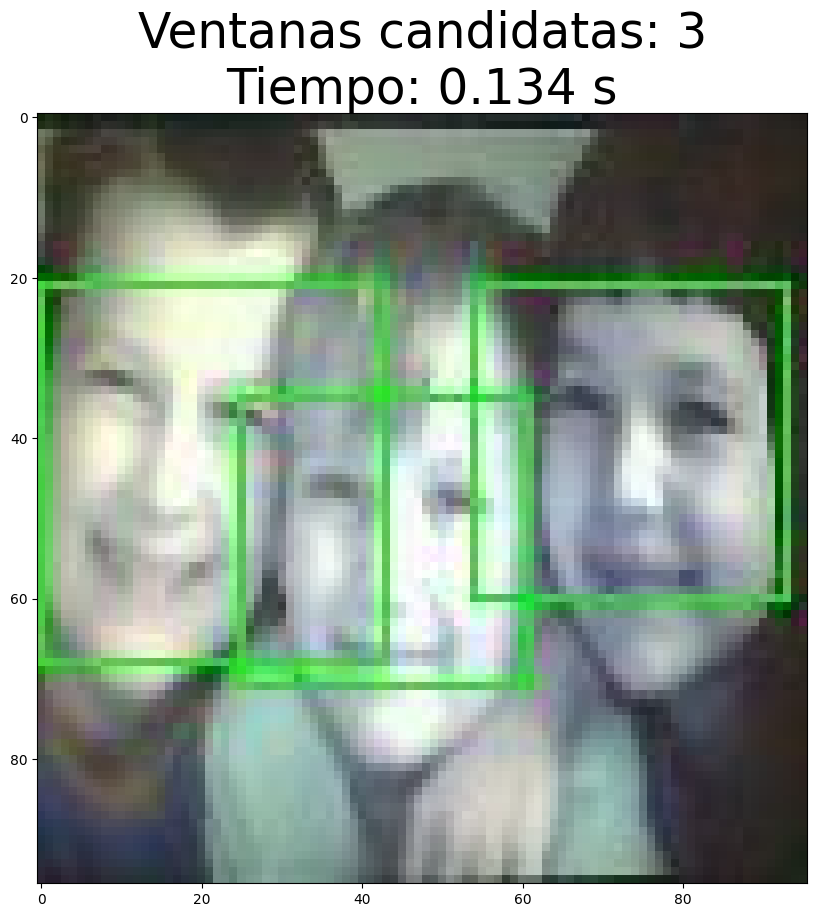
\includegraphics[width=\textwidth]{./Figures/rnet.png}
         \caption{R-Net postprocesado.}
         \label{fig:2de3}
     \end{subfigure}
     \hfill
	 \begin{subfigure}[b]{0.28\textwidth}
         \centering
         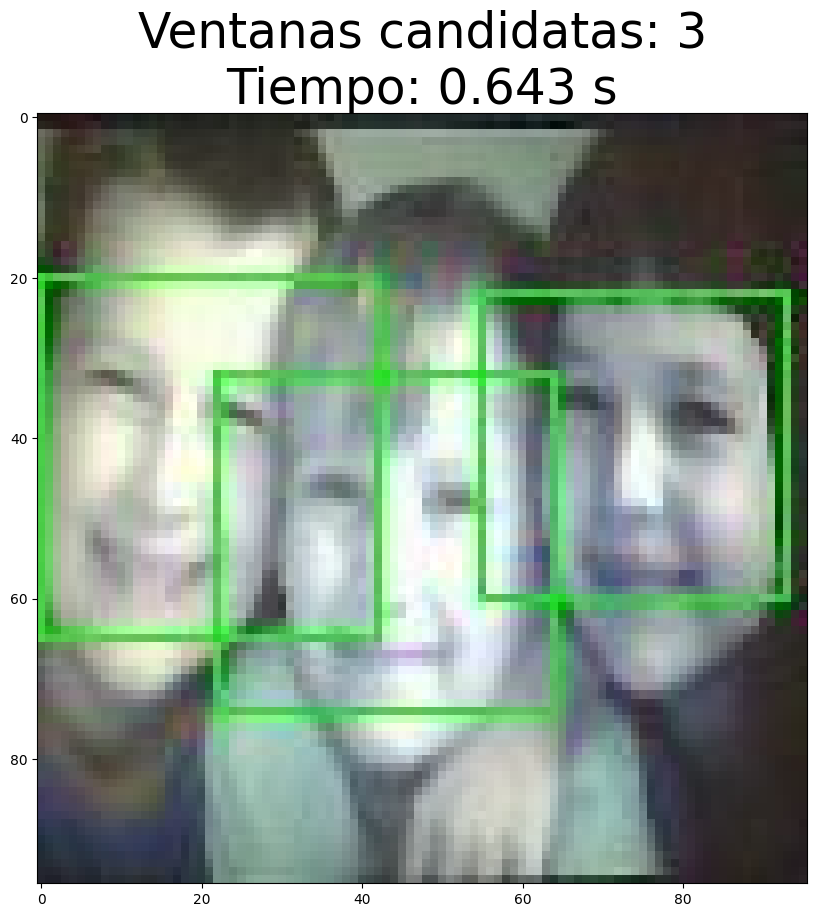
\includegraphics[width=\textwidth]{./Figures/onet.png}
         \caption{O-Net postprocesado.}
         \label{fig:2de3}
     \end{subfigure}
     \hfill
        \caption{Resultados para TensorFlow Lite Micro con cuantización a 8 bits.}
        \label{fig:test_tflm}
\end{figure}

Los resultados obtenidos de las pruebas en Google Colab fueron los esperados. A medida que los modelos se iban optimizando en tamaño y tiempo de respuesta, la precisión de los resultados se reducía. Para las pruebas realizadas sobre el prototipo de pruebas, los resultados también estuvieron acordes a lo planeado, si bien el tamaño es el más pequeño posible, los tiempos de inferencia son mucho más altos que para los modelos probados en Google Colab, esto por las limitaciones de hardware del ESP32-S3, aun así los resultados finales son muy similares. En la tabla \ref{tab:test_tf_models} se exponen los resultados para todas las pruebas sobre los modelos.

\begin{table}[h]
	\centering
	\caption[Resultados de las pruebas sobre los modelos]{Resultados de las pruebas sobre los modelos}
	\begin{tabular}{lcc}   
		\toprule
		\textbf{Modelo} & \textbf{Rostros encontrados} & \textbf{Tiempo de ejecución MTCNN (ms)} \\
		\midrule
		TF & 3 & 456 \\
		TF Lite & 3 & 14 \\
		TF Lite 8 bits & 3 & 19 \\
		TF Lite Micro 8 bits & 3 & 842 \\
		\bottomrule
		\hline
	\end{tabular}
	\label{tab:test_tf_models}
\end{table}

%----------------------------------------------------------------------------------------
% SECTION 3
%----------------------------------------------------------------------------------------
\section{Pruebas sobre el sensor de movimiento}
Las pruebas realizadas sobre el sensor de movimiento tuvieron el objetivo de determinar el comportamiento de las señales de salida generadas por el TLV8544 cuando se genera movimiento en el rango de acción del sensor PIR. Para este fin se conectaron las sondas del osciloscopio en la salida de la señal analógica y en las 2 salidas digitales de los comparadores. En la figura \ref{fig:test_pir} se observan las señales capturadas por el osciloscopio para 5 movimientos detectados por el sensor PIR.

\begin{figure}[h]
	\centering
	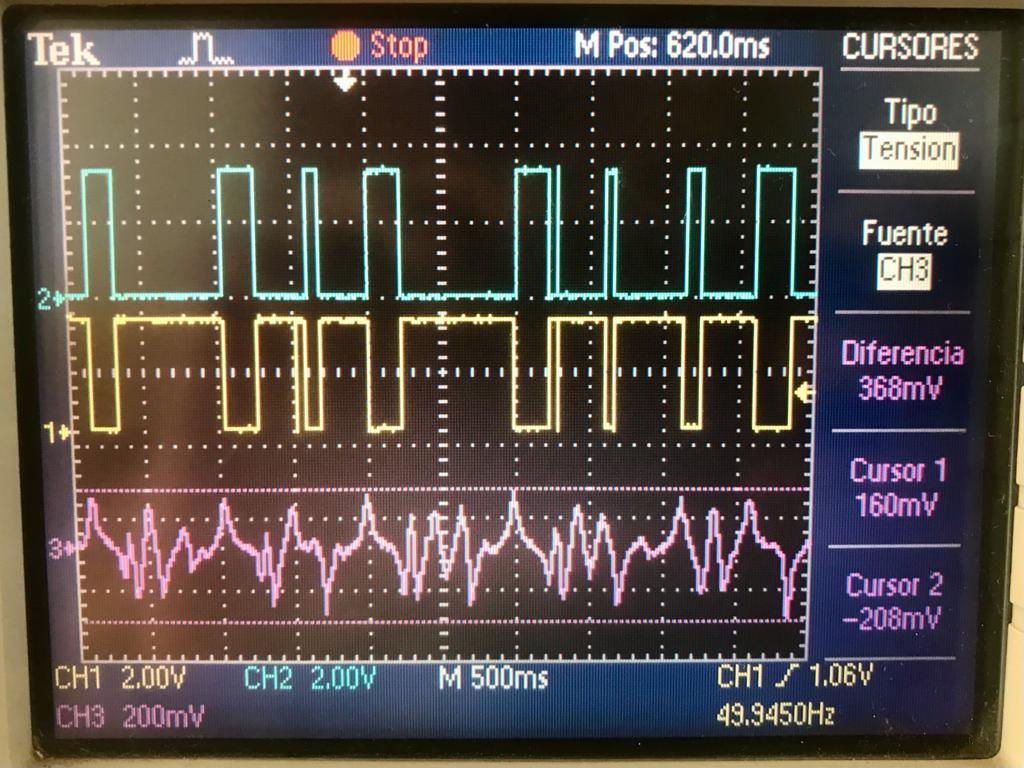
\includegraphics[scale=0.3]{./Figures/test_pir.jpeg}
	\caption{Señales de salida del sensor de movimiento.}
	\label{fig:test_pir}
\end{figure}

Como se puede observar de la figura \ref{fig:test_pir} se generaron señales de corta duración que causaron falsos positivos en la detección de movimiento. Este efecto fue subsanado con la ayuda de una máquina de estados implementada en el programa que corre el coprocesador ULP.

%----------------------------------------------------------------------------------------
% SECTION 4
%----------------------------------------------------------------------------------------
\section{Pruebas de consumo energético sobre el sistema}
Estas pruebas consistieron en poner en funcionamiento el prototipo de pruebas y medir el consumo de corriente para determinar si todas las técnicas de bajo consumo fueron aplicadas correctamente. Como se mostró en la figura \ref{fig:ulp_modes} el sistema durante su funcionamiento realiza transiciones entre 3 estados distintos, donde cada estado tiene un consumo de corriente diferente. Con ayuda del PPK2 y del software nRF Connect for Desktop con su módulo Power Profile, se midió el consumo de corriente del sistema durante un tiempo de 5 minutos, donde fue activado en varias ocasiones mediante el sensor de movimiento. En la figura \ref{fig:test_ulp2} se observa un gráfico donde se puede apreciar el comportamiento del sistema a través de la forma en como cambia su consumo de corriente con relación al tiempo.

\begin{figure}[h]
	\centering
	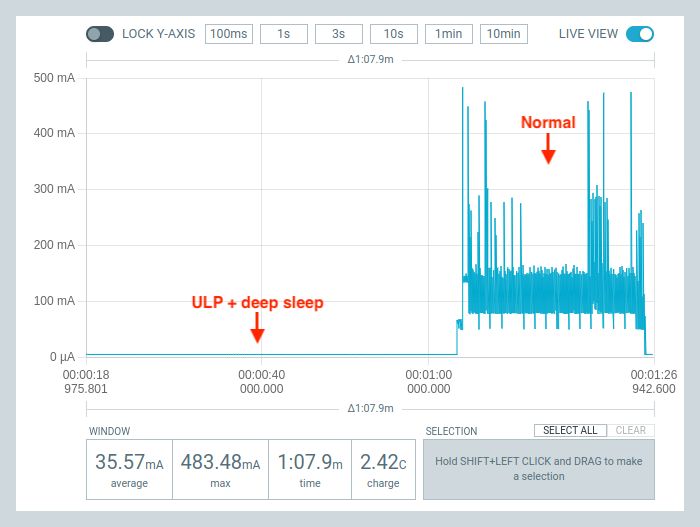
\includegraphics[scale=0.45]{./Figures/test_ulp1.png}
	\caption{Gráfico de consumo de corriente del sistema.}
	\label{fig:test_ulp1}
\end{figure}

La figura \ref{fig:test_ulp1} muestra el 1 ciclo de trabajo normal, es decir, que se mantiene en modo de bajo consumo hasta que detecta un movimiento válido mediante el sensor de movimiento y activa el procesador principal para realizar las tareas de detección facial y comunicación con los servicios en la nube. Cuando el dipositivo se encuentra en modo de bajo consumo cambia entre los estados Deep sleep y ULP cada 100 ms, donde en el estado ULP se ejecuta la máquina de estados que mitiga los errores causados por los falsos positivos generados por el sensor de movimiento. En la figura \ref{fig:test_ulp2} se exhibe con mayor detalle el funcionamiento cuando el dispositivo se encuentra en modo de bajo consumo.

\clearpage


\begin{figure}[h]
	\centering
	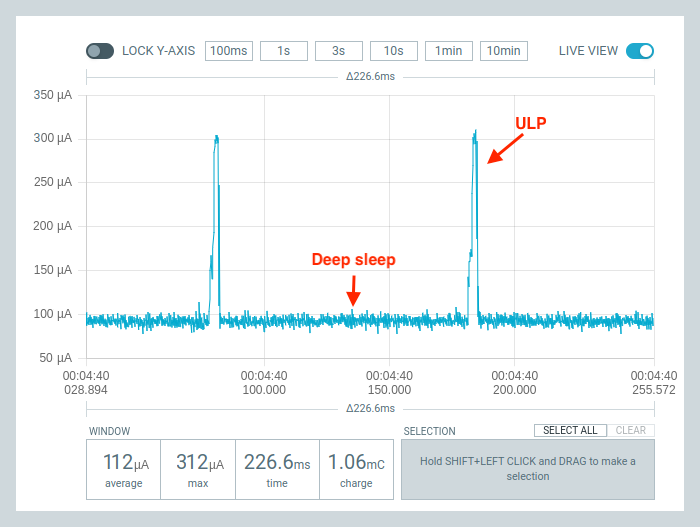
\includegraphics[scale=0.45]{./Figures/test_ulp2.png}
	\caption{Gráfico de consumo de corriente del sistema.}
	\label{fig:test_ulp2}
\end{figure}

En la tabla \ref{tab:test_ulp} se detallan los consumos de corriente y los tiempos de duración de todos los estados de consumo del dispositivo.

\begin{table}[h]
	\centering
	\caption[Consumo de corriente del dispositivo]{Consumo de corriente aproximado de todos los modos del dispositivo}
	\begin{tabular}{lccc}   
		\toprule
		\textbf{Estado} & \textbf{Consumo promedio (mA)} & \textbf{Consumo máximo (mA)} & \textbf{Tiempo (s)} \\
		\midrule
		Normal & 97.31 & 478.21 & 22.8 \\
		ULP & 0.247 & 0.310 & 0.003 \\
		\textit{Deep sleep} & 0.014 & 0.017 & 0.1 \\
		\bottomrule
		\hline
	\end{tabular}
	\label{tab:test_ulp}
\end{table}

El evento que despierta al procesador principal para ejecutar las tareas de detección facial y comunicación con los servicios en la nube es asíncrono, es decir, que no es posible predecirlo y puede ocurrir muchas veces o muy pocas, por lo que no es posible medir una corriente promedio del dispositivo en general y por tanto tampoco se pudo establecer el tiempo que un par de baterías de litio AA podría alimentar el dispositivo.

%----------------------------------------------------------------------------------------
% SECTION 5
%----------------------------------------------------------------------------------------
\section{Pruebas sobre los servicios en la nube}
Las pruebas sobre los servicios en la nube se basaron en simular la conexión y publicación de mensajes de 3 dispositivos distintos por un lapso de 10 minutos. La simulación de los dispositivos se hizo con ayuda del \textit{script} de Python mostrado en \ref{cod:test_iot}, que tiene la función de conectarse al broker de Iot Core y publicar 15 mensajes en un lapso 15 minutos para cada uno de los dispositivos a simular.

\begin{lstlisting}[language=Python, label=cod:test_iot, caption=Código del \textit{script} para probar IoT Core.]
from random import random
from awscrt import mqtt
from awsiot import mqtt_connection_builder
import time as t
import random

ENDPOINT = "xxxxxxxxxxxxxxxxxxxxxxxxxxxxxxx.amazonaws.com"
CLIENT_ID = "dev1"
PATH_TO_CERTIFICATE = "dev_cert.pem.crt"
PATH_TO_PRIVATE_KEY = "priv_key.pem.key"
PATH_TO_AMAZON_ROOT_CA_1 = "AmazonRootCA1.pem"
TOPIC = "faceCounter"

mqtt_connection = mqtt_connection_builder.mtls_from_path(endpoint=ENDPOINT, cert_filepath=PATH_TO_CERTIFICATE, pri_key_filepath=PATH_TO_PRIVATE_KEY, ca_filepath=PATH_TO_AMAZON_ROOT_CA_1, client_id=CLIENT_ID, clean_session=False, keep_alive_secs=6)

# Device IDs
id = ["7a5b4c79-621d-476d-83b4-861005589752", "8a5b4c79-621d-476d-83b4-861005589752", "9a5b4c79-621d-476d-83b4-861005589752"]

# Connect to broker
connect_future = mqtt_connection.connect()
connect_future.result()

# Send messages for all IDs
for i in range(30):
    for j in id:
        # Set new values for the JSON message
        message = "{\n\"id\":\"%s\",\n\"payload\":{\n\"faces\":%d,\n\"battery\":%d,\n\"temperature\":%d\n}\n}" % (j, random.randint(0, 5), random.randint(50, 90), random.randint(19, 27))
        mqtt_connection.publish(topic=TOPIC, payload=message, qos=mqtt.QoS.AT_LEAST_ONCE)
    # Wait for 1 min
    t.sleep(60)

# Disconnect from broker
disconnect_future = mqtt_connection.disconnect()
disconnect_future.result()
\end{lstlisting}

Para controlar los mensajes que son recibidos por el \textit{broker} se utilizó el monitor MQTT de IoT Core MQTT Test, que consiste en un cliente que puede publicar y suscribirse a uno o varios tópicos. En la figura \ref{fig:test_iot} se observa un mensaje publicado por el \textit{script} del código \ref{cod:test_iot} en el tópico \texttt{faceCounter}.

\begin{figure}[h]
	\centering
	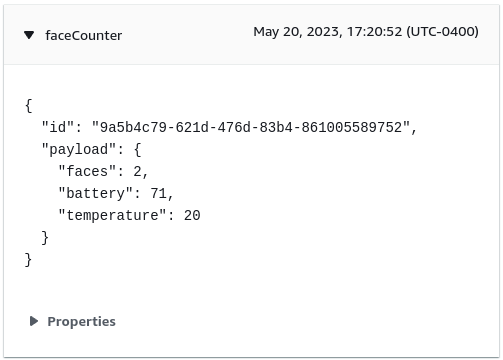
\includegraphics[scale=0.45]{./Figures/test_iot.png}
	\caption{Mensaje de prueba recibido en MQTT Test Client.}
	\label{fig:test_iot}
\end{figure}

Los mensajes publicados en \texttt{faceCounter} fueron procesados mediante un \textit{rule} para grabar los datos de relevancia en la tabla \texttt{faceCounter} de la base de datos \texttt{iot} de Timestream. El código \ref{cod:test_sql} consulta los datos de los últimos 5 minutos de  de la tabla \texttt{faceCounter} y en la figura \ref{fig:test_timestream} se muestran los resultados obtenidos.

\begin{lstlisting}[language=SQL, label=cod:test_sql, caption=Código SQL para obtener los datos de la tabla faceCounter.]
SELECT * FROM "iot"."faceCounter" WHERE time between ago(5m) and now() ORDER BY time 
\end{lstlisting}

\begin{figure}[h]
	\centering
	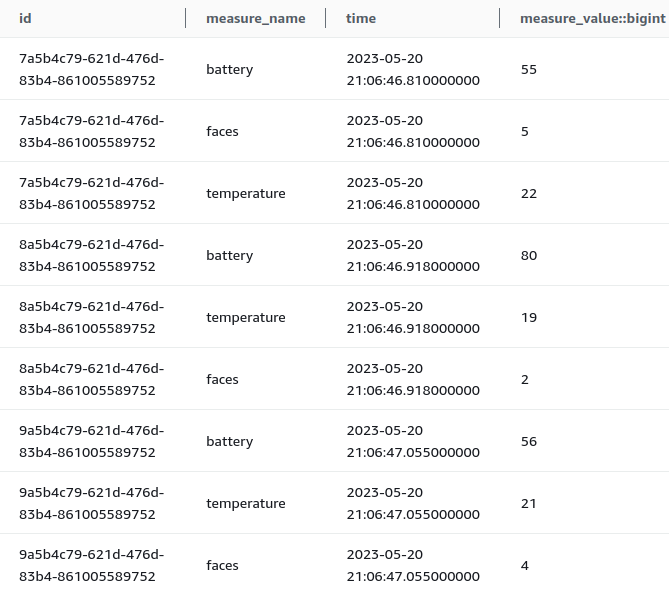
\includegraphics[scale=0.45]{./Figures/test_timestream.png}
	\caption{Tabla faceCounter con los datos de prueba.}
	\label{fig:test_timestream}
\end{figure}

Finalmente, en la figura \ref{fig:test_dashboard} se exhibe el \textit{dashboard} creado con Grafana, donde cada columna representa mediante gráficos los datos de uno de los dispositivos simulados.
\begin{figure}[h]
	\centering
	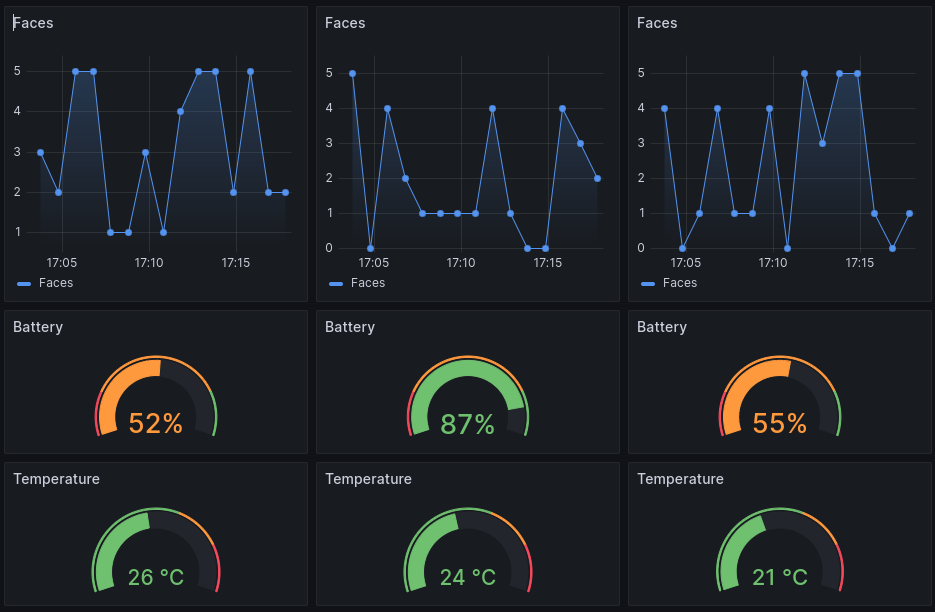
\includegraphics[scale=0.3]{./Figures/test_dashboard.png}
	\caption{\textit{Dashboard} con datos de prueba para 3 dispositivos.}
	\label{fig:test_dashboard}
\end{figure}
